% !TeX root = Thesis.tex

\begin{figure}[ht]
    \centering
    \begin{subfigure}{0.28\textwidth}
        \centering
        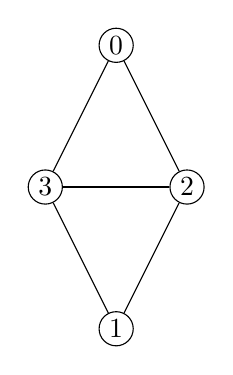
\begin{tikzpicture}[
            scale=0.9,
            every node/.style={
                circle,
                draw,
                fill=white,
                inner sep=1.5pt
            }
        ]
            \node (0) at (0,2) {$0$};
            \node (3) at (-1,0) {$3$};
            \node (2) at (1,0) {$2$};
            \node (1) at (0,-2) {$1$};

            \draw (0)--(3);
            \draw (0)--(2);
            \draw (3)--(2);
            \draw (3)--(1);
            \draw (2)--(1);
        \end{tikzpicture}
        \caption{$G$}
        \label{fig::fundamental_example_graph}
    \end{subfigure}
    \hfill
    \begin{subfigure}{0.28\textwidth}
        \centering
        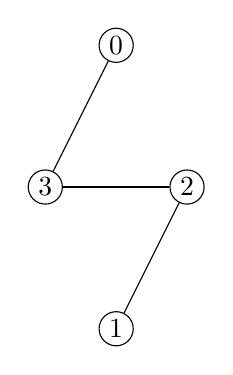
\begin{tikzpicture}[
            scale=0.9,
            every node/.style={
                circle,
                draw,
                fill=white,
                inner sep=1.5pt
            }
        ]
            \node (0) at (0,2) {$0$};
            \node (3) at (-1,0) {$3$};
            \node (2) at (1,0) {$2$};
            \node (1) at (0,-2) {$1$};

            \draw (0)--(3);
            \draw (3)--(2);
            \draw (2)--(1);
        \end{tikzpicture}
        \caption{$T_1$}
        \label{fig::fundamental_example_root_1}
    \end{subfigure}
    \hfill
    \begin{subfigure}{0.28\textwidth}
        \centering
        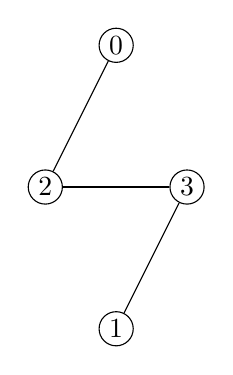
\begin{tikzpicture}[
            scale=0.9,
            every node/.style={
                circle,
                draw,
                fill=white,
                inner sep=1.5pt
            }
        ]
            \node (0) at (0,2) {$0$};
            \node (2) at (-1,0) {$2$};
            \node (3) at (1,0) {$3$};
            \node (1) at (0,-2) {$1$};

            \draw (0)--(2);
            \draw (2)--(3);
            \draw (3)--(1);
        \end{tikzpicture}
        \caption{$T_2$}
        \label{fig::fundamental_example_root_2}
    \end{subfigure}

    \caption{The graph $G$ has two possible $P_4$ square roots that are trees, $T_1$ and $T_2$. The two roots are isomorphic, differing only by the interchange of vertices $2$ and $3$.}
    \label{fig::fundamental_example}
\end{figure}